\chapter{Theory}
\section{The Model Organism/Study Animal}
Euryhaline, osmoconformer, closes valves in periods of exposure to brackish/fresh water (low tide), keeping the saline pallial/mantle fluid as the immediate surrounding environment. Becomes isosmotic with the pallial fluid (Gilles, 1972). In long exposures (> 75 hours) or by puncturing/keeping the valves prised they are forced to pump water, and the hemolymph rapidly conforms to the exterior osmolarity. Short said: is an osmoconformer that behaviorally protects itself from short-term exposures to hypo-osmotic conditions rather than physiologically (Davenport, 1979). Relevant for the osmolarity of buffers/solutions used.

\begin{figure}[H]
    \centering
    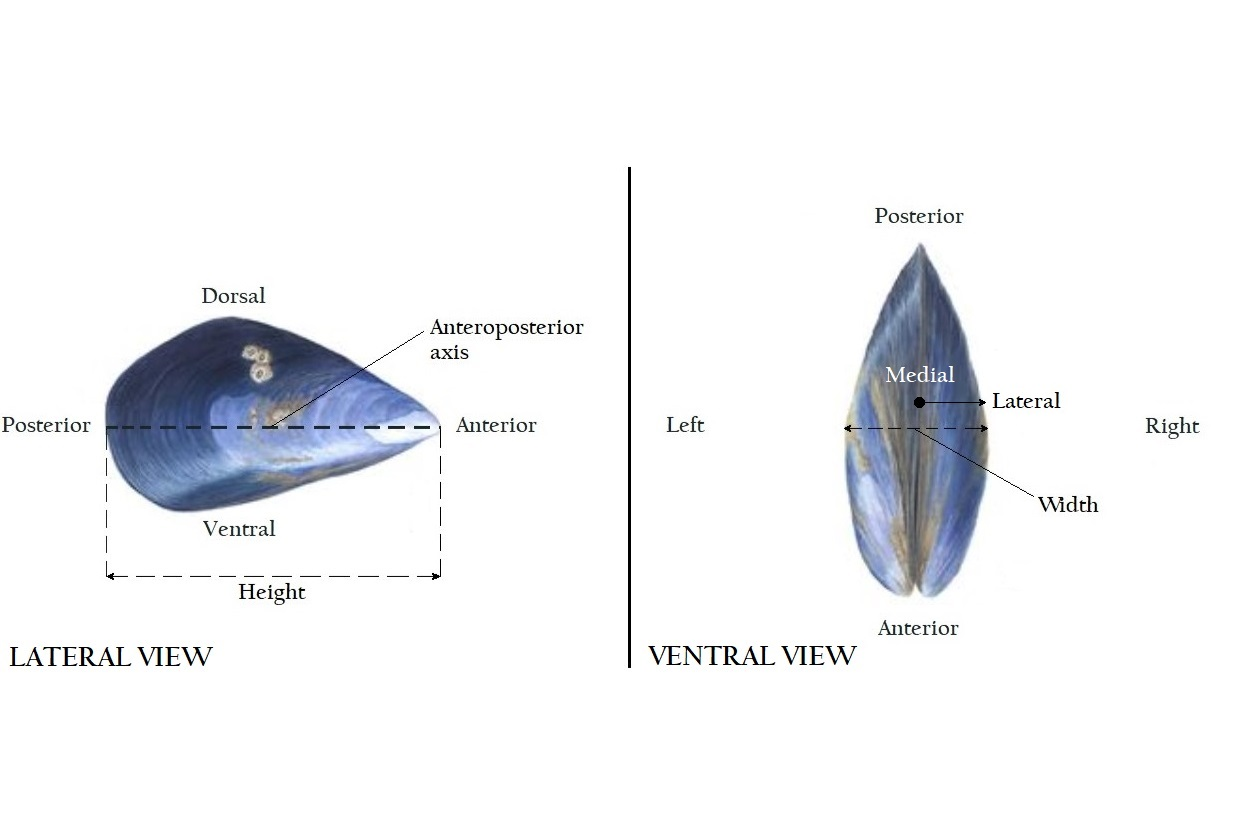
\includegraphics[width=\textwidth]{figures/Anatomy/M_edulis_anatomical_axis_lateral.jpg}
    \caption{The figure caption depends on if it ends up here, or in the material and method. Write when decided. The illustration was adapted from an artistic work by Abby Towne, A. Towne Design with permission.}
    \label{fig:anatomical_axis}
\end{figure}

\section{The role of hemocytes}
Hemocytes also (in addition to lung and digestive gland) showed high expression levels (of initiator and executioner caspases), probably due to the role of apoptosis in the defense against pathogens. Because bivalves are highly susceptible to climate changes, pollutants and pathogens, it  could be suggested that a strong apoptotic process may be necessary to ensure body homeostasis. (Romero, 2011). See page 11 of (New Insights into the Apoptotic Process in Mollusks: Characterization of Caspase Genes in Mytilus galloprovincialis) for greater detail and references.

Relocate the article about the role of hemocytes in wound-healing in mussels.